%!TEX root = ../../main.tex

\graphicspath{{../../figures/appendix/}}

\chapter{Pattern classification}
\label{ch:cell_pattern_classification}

\newpage

\section{t-SNE representations of the pattern classification}
\label{sec:tsne_classification}

\begin{center}
	\textit{(To be completed)}
\end{center}

\vfill

\begin{figure}[h]
	\centering
	\minipage{0.2\textwidth}
		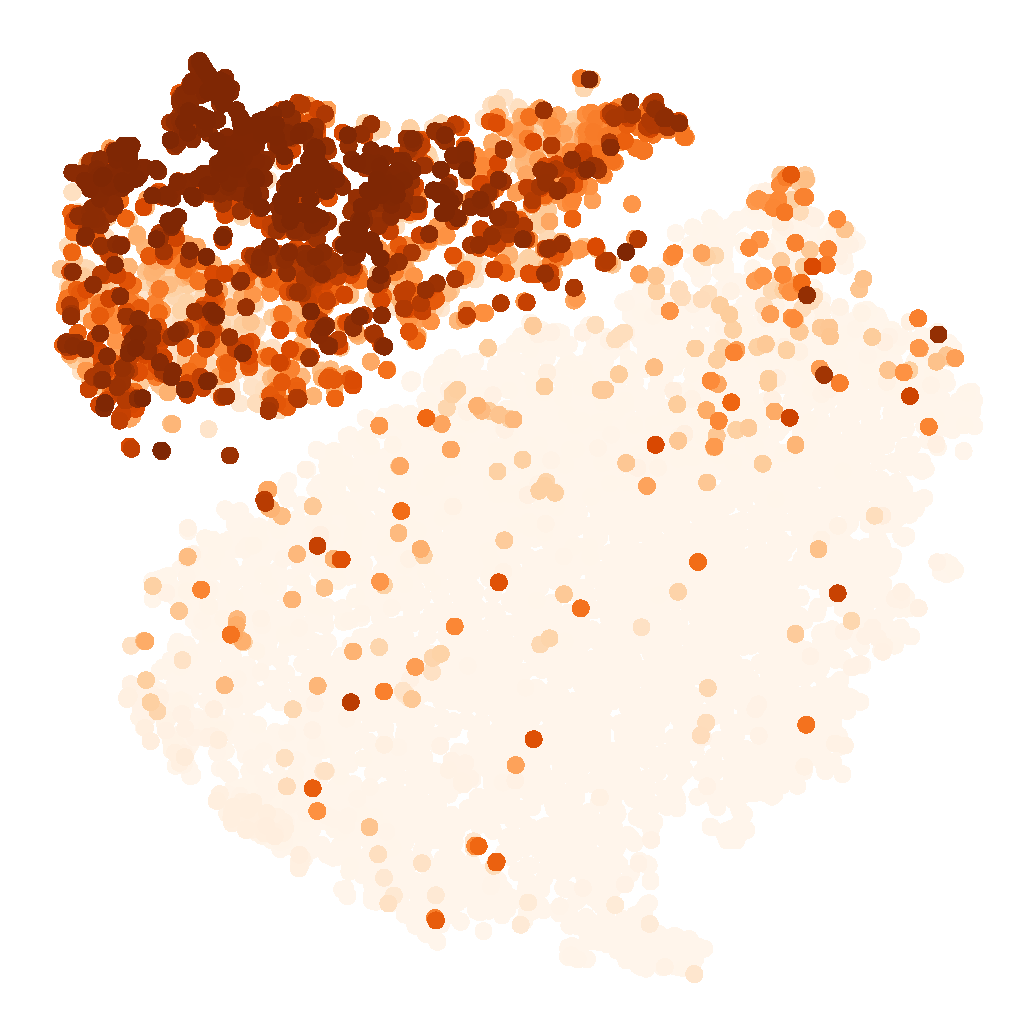
\includegraphics[width=\linewidth]{figures/appendix/tsne_probability_nocolorbar_foci}
		\subcaption{Foci}
		\vfill
		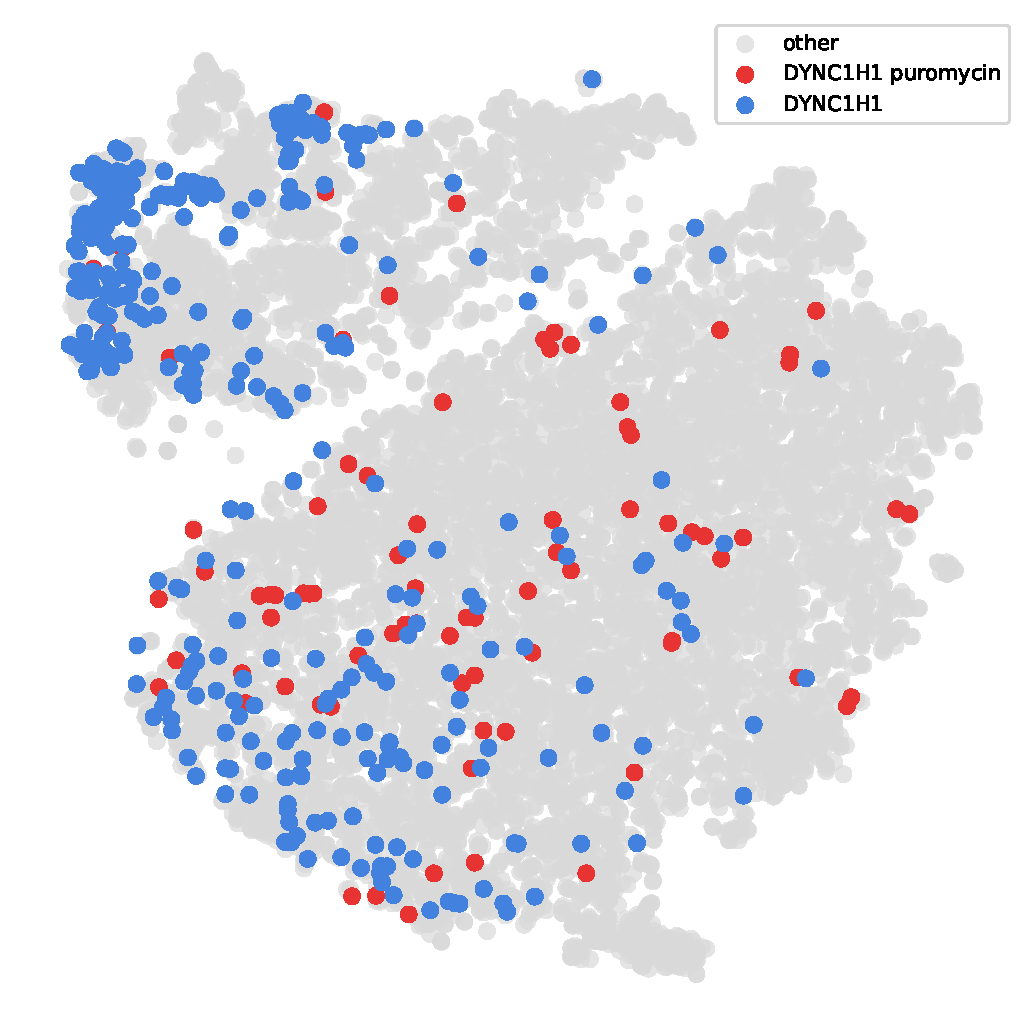
\includegraphics[width=\linewidth]{figures/appendix/tsne_foci_DYNC1H1}
		\subcaption{DYNC1H1}
	\endminipage\hfill
	\minipage{0.2\textwidth}
		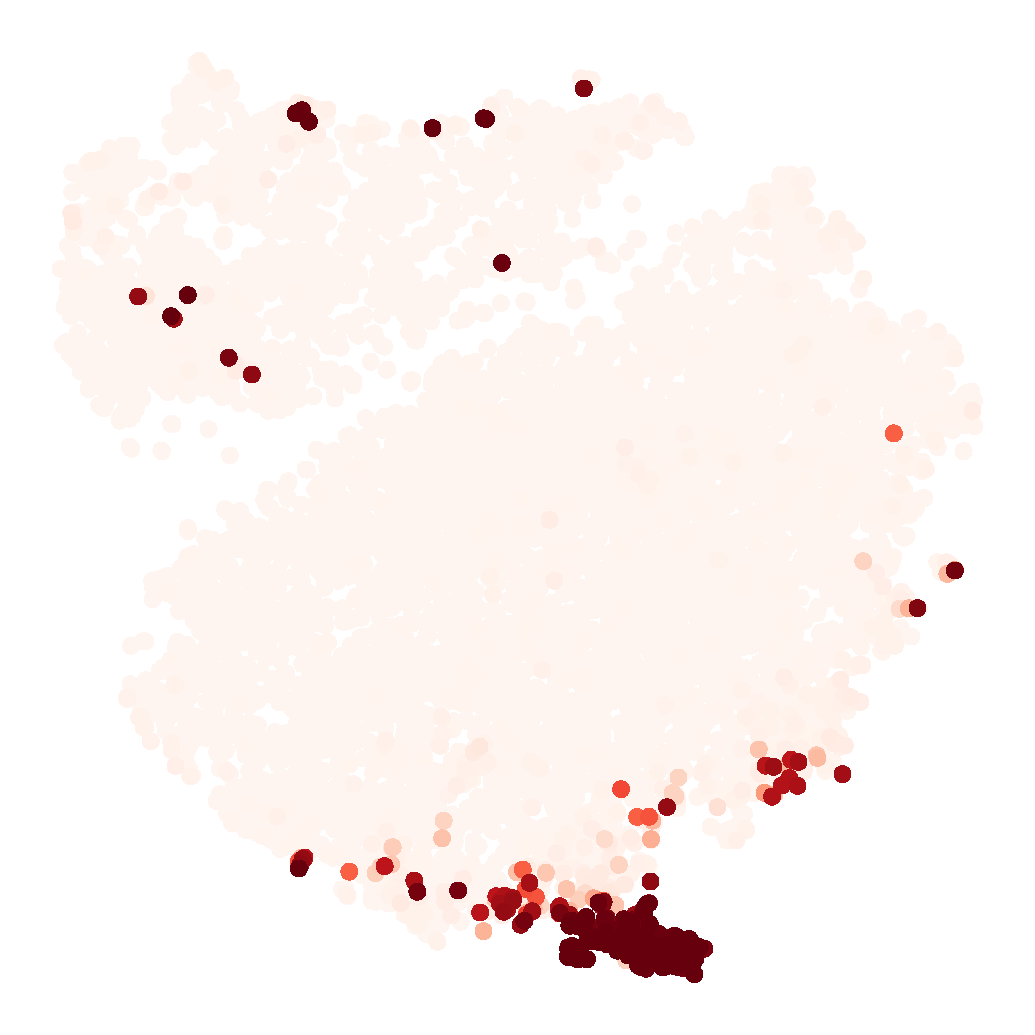
\includegraphics[width=\linewidth]{figures/appendix/tsne_probability_nocolorbar_intranuclear}
		\subcaption{Intranuclear}
		\vfill
		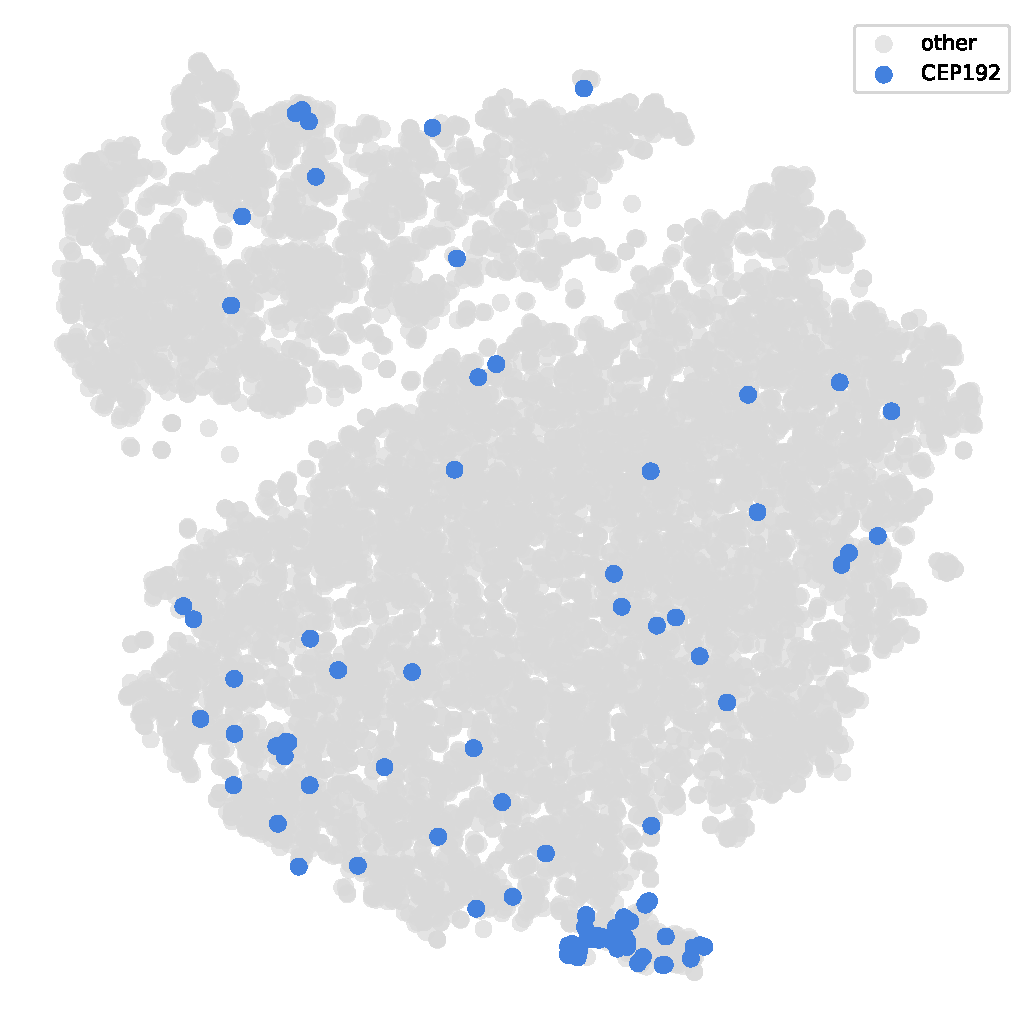
\includegraphics[width=\linewidth]{figures/appendix/tsne_intranuclear_CEP192}
		\subcaption{CEP192}
	\endminipage\hfill
	\minipage{0.2\textwidth}
		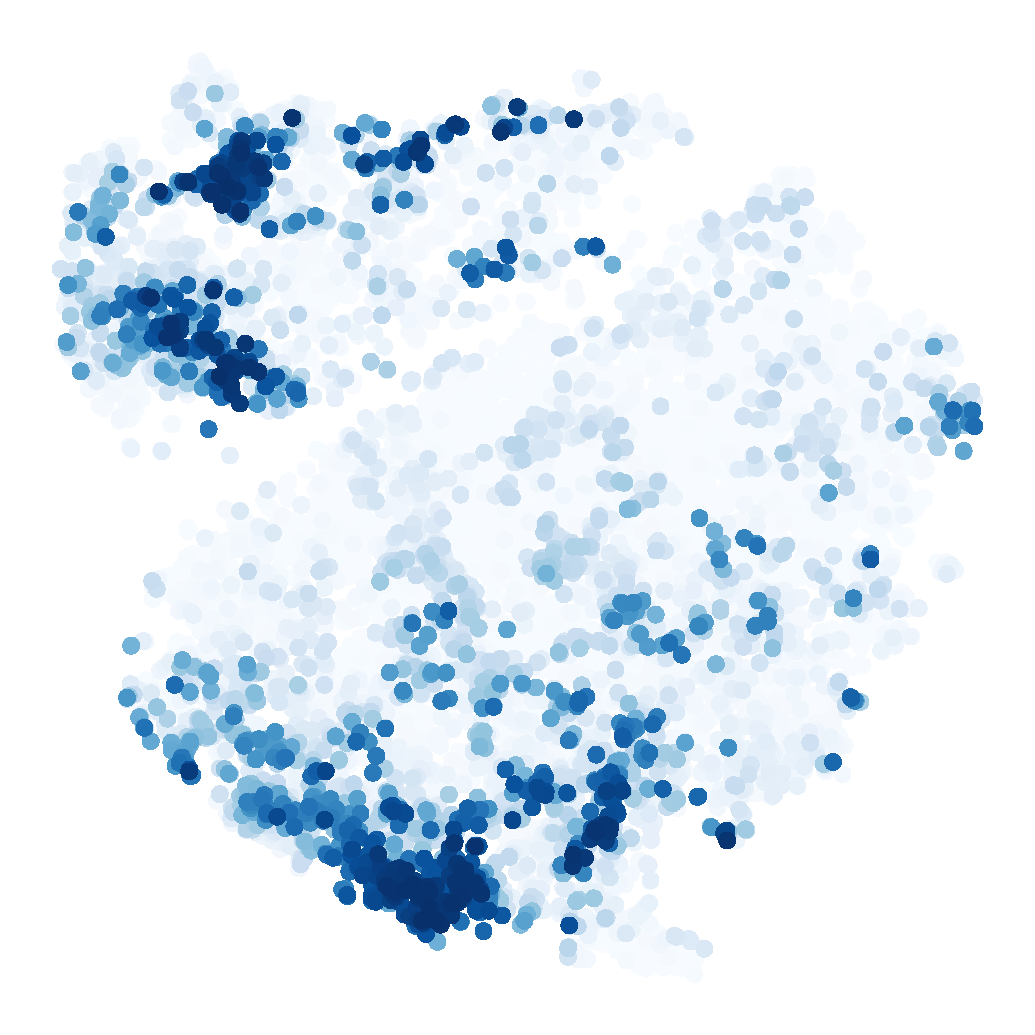
\includegraphics[width=\linewidth]{figures/appendix/tsne_probability_nocolorbar_nuclear}
		\subcaption{Nuclear edge}
		\vfill
		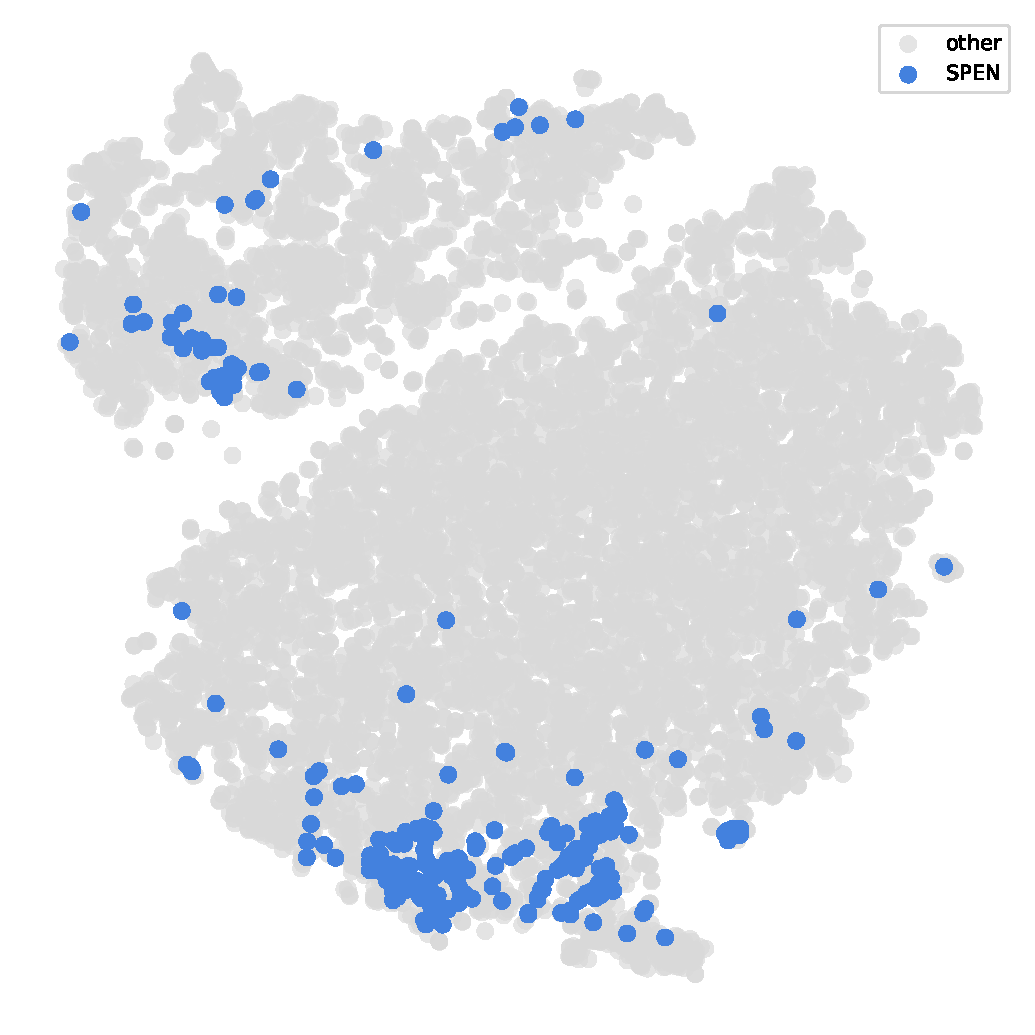
\includegraphics[width=\linewidth]{figures/appendix/tsne_nuclear_SPEN}
		\subcaption{SPEN}
	\endminipage\hfill
	\minipage{0.2\textwidth}
		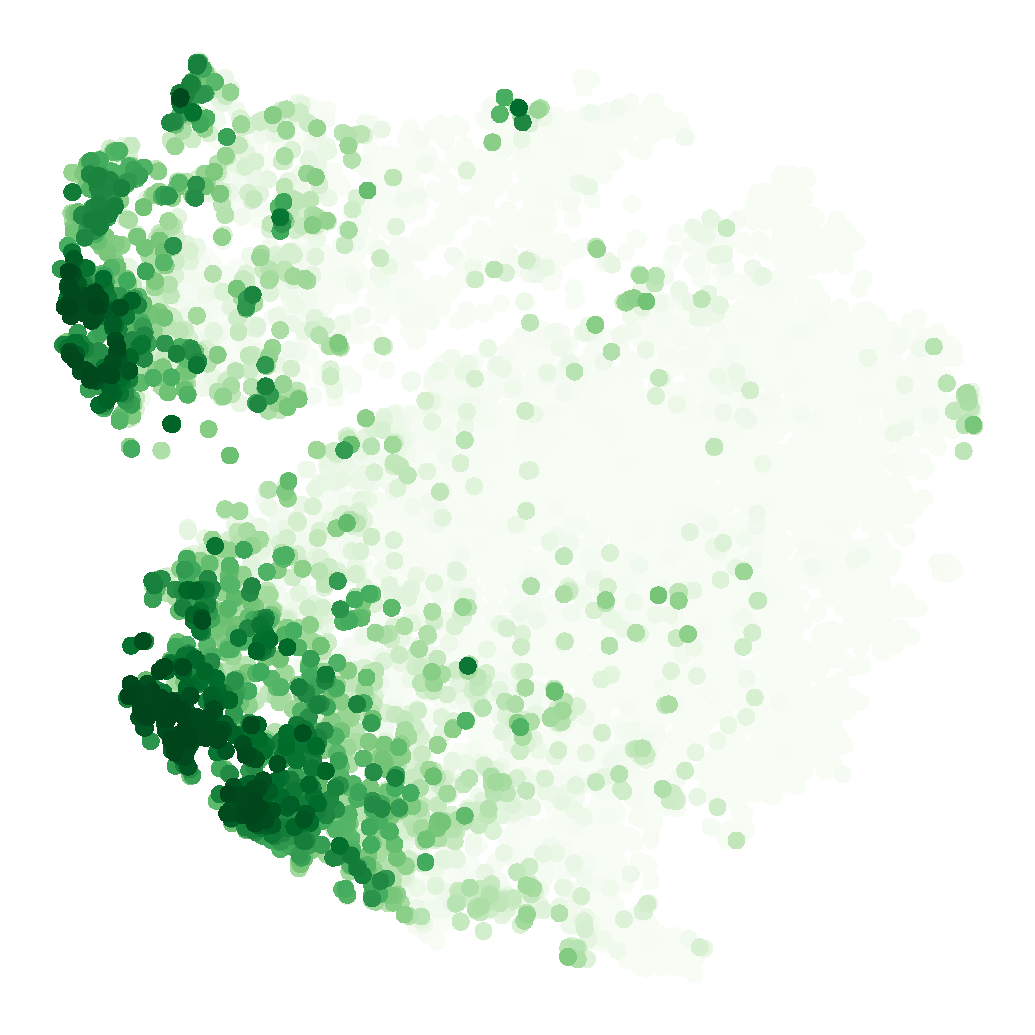
\includegraphics[width=\linewidth]{figures/appendix/tsne_probability_nocolorbar_perinuclear}
		\subcaption{Perinuclear}
		\vfill
		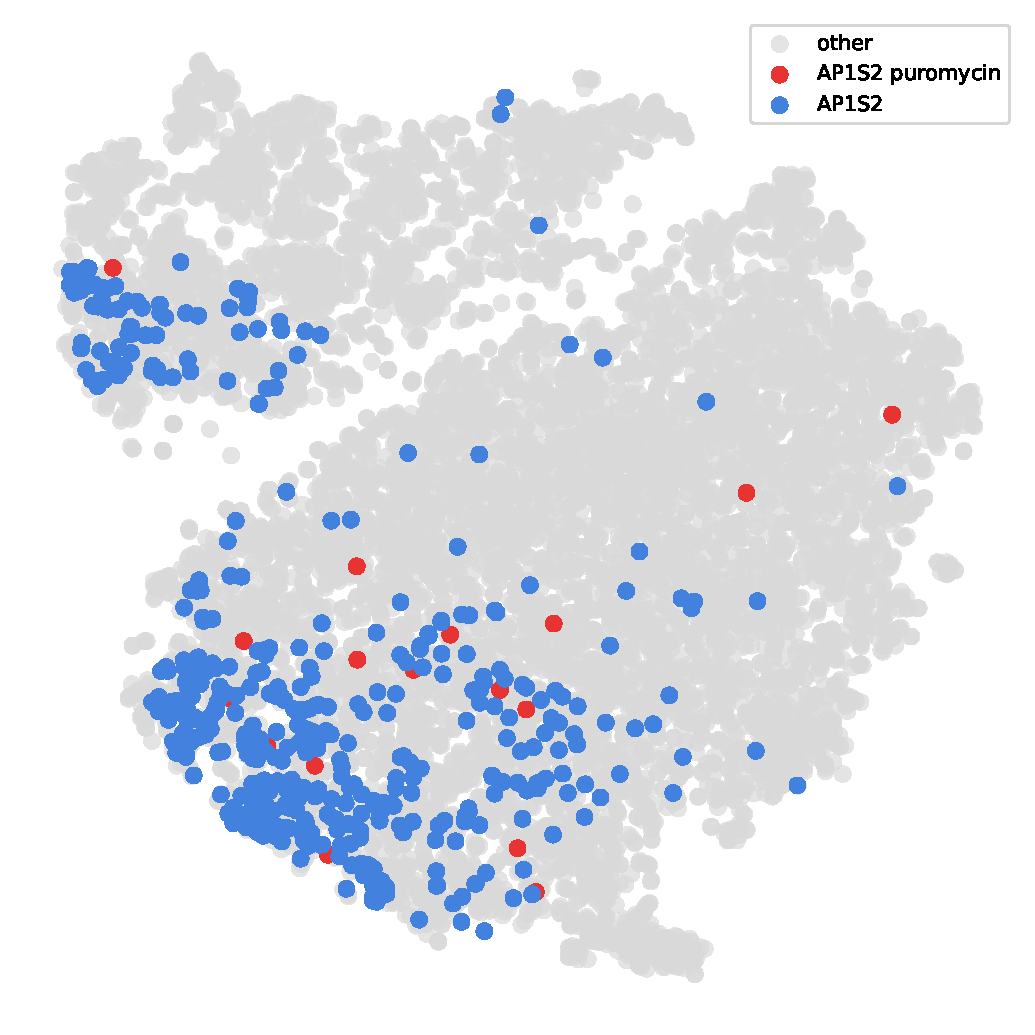
\includegraphics[width=\linewidth]{figures/appendix/tsne_perinuclear_AP1S2}
		\subcaption{AP1S2}
	\endminipage\hfill
	\minipage{0.2\textwidth}
		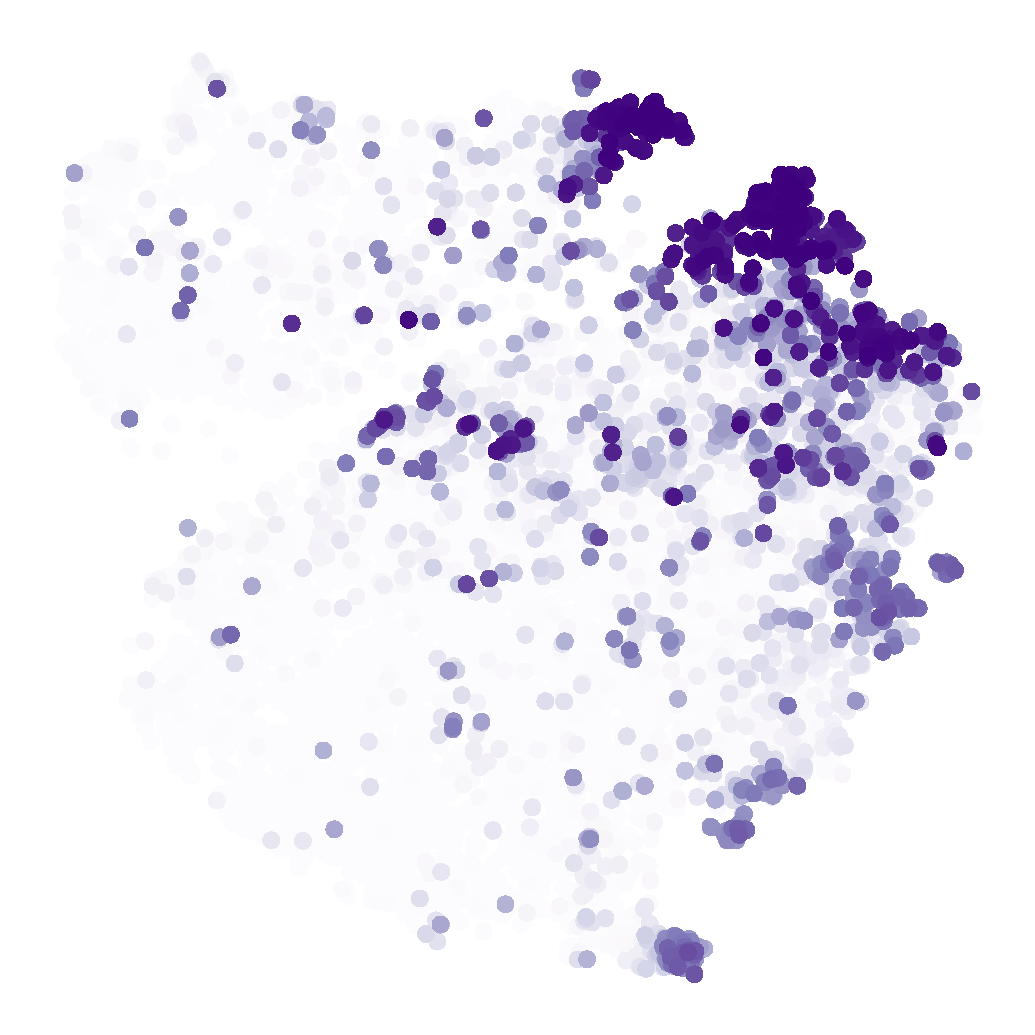
\includegraphics[width=\linewidth]{figures/appendix/tsne_probability_nocolorbar_protrusion}
		\subcaption{Protrusion}
		\vfill
		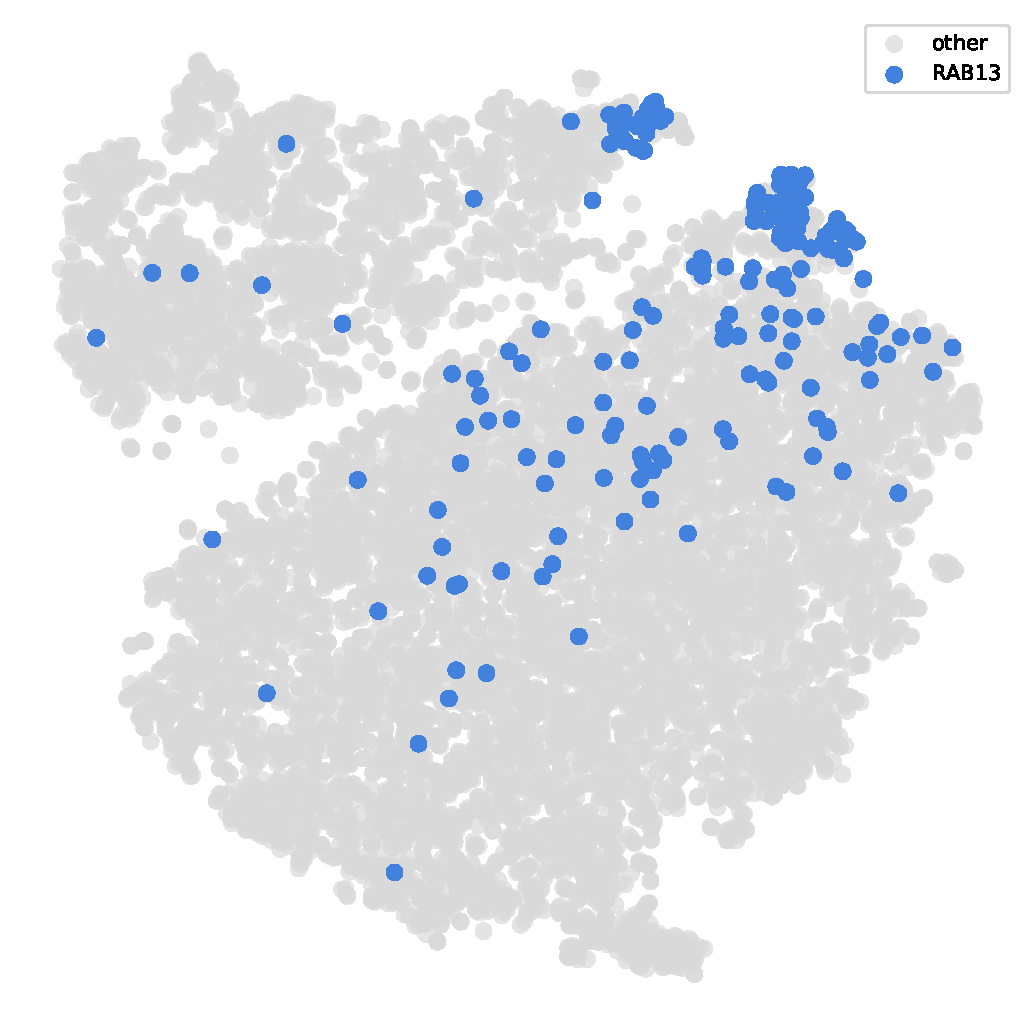
\includegraphics[width=\linewidth]{figures/appendix/tsne_protrusion_RAB13}
		\subcaption{RAB13}
	\endminipage
	\caption{(\textit{Top}) Visualization of random forest classification probabilities in the t-SNE, from~\cite{CHOUAIB_2020}.
	Color indicates the probabilities of the cell to be classified in the indicated localization pattern.
	The darker, the higher the probability is.
	(\textit{Bottom}) Visualization of cells for some specific genes with the indicated localization pattern above.
	Cells can be untreated (\textit{blue}) or treated with puromycin (\textit{red})}
	\label{fig:tsne_proba_gene}
\end{figure}

%Figure~\ref{fig:tsne_proba_gene}

% classifications-probability matche annotations in tsne
% consistent with observation on the genes
% noise at the gene level
% impact of puromycin seen on the tsne

\vfill

\newpage

\section{Cell-wise pattern heterogeneity}
\label{sec:pattern_heterogeneity}

\begin{center}
	\textit{(To be completed)}
\end{center}

\vfill

\begin{figure}[h]
    \centering
    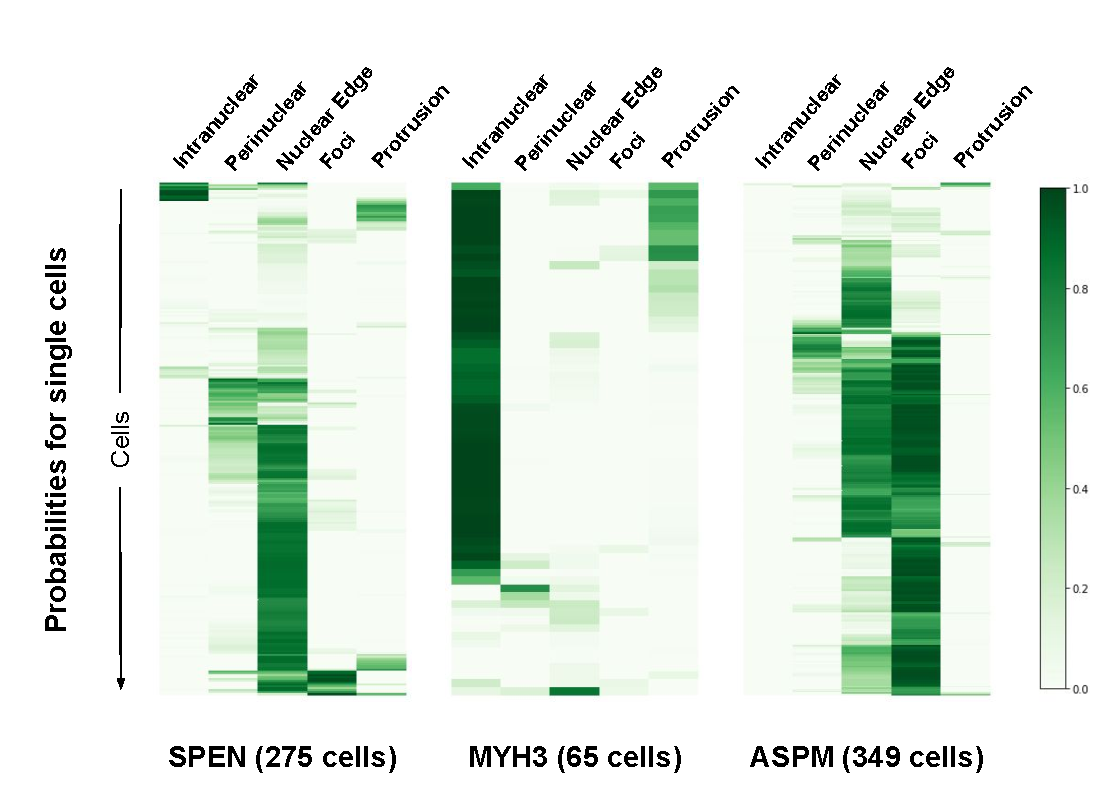
\includegraphics[width=\textwidth]{figures/appendix/heatmap_cell_racha}
    \caption{Three heat maps from~\cite{CHOUAIB_2020} with the probability of single cells to have each patterns.
	Only cells where we visualized SPEN, MYH3 and ASPM transcripts are represented.
	Each row corresponds to a cell and the color indicates the probabilities of the cell to be classified in the indicated localization pattern}
    \label{fig:heatmap_racha_cells}
\end{figure}

%Figure~\ref{fig:heatmap_racha_cells}

% noiseatthe gene level
% alot of heterogeneity for the same gene
% some cell return a high probability for several patterns at the same time

\vfill